\section{Standalone WAGASCI-module performances}
\label{sec:mc_study_standalone}

%%%%%%%%%%%%%%%%%%%%%%%%%%%%%%%%%%%
In the previous sections, the WAGASCI detector was studied using the Muon Range Detectors. In this section, the standalone abilities of WAGASCI module are presented. 
Using the WAGASCI configuration presented in Section~\ref{sec:mc_study}, we have evaluated that only $7\%$ of the muons will be stopped in one of the WAGASCI modules. 
However, this proportion increases to $53\%$ for pions and $73\%$ for protons produced by neutrino interactions at $1.5^{\circ}$ off-axis. Figure~\ref{fig:stoppedproportions} shows the momentum distribution of these daughter particles as well as for the sub-sample stopped in one of the WAGASCI modules. 
Therefore, the study of the standalone abilities of the WAGASCI module in this section are dominantly motivated by:
\begin{itemize}
\item the accurate measurement of the neutrino interaction final states. Though most of the muons will be reconstructed and identified in the MRDs, the hadronic particles will predominantly stops in one WAGASCI module. One has therefore to rely exclusively on the WAGASCI module information alone to reconstruct, identify and measure the momentum of pions or protons.
\item the coverage of the MRDs is not $4\pi$. Using the WAGASCI module information can therefore help to constraint the particles that exits the WAGASCI module but do not geometrically enters any MRD.
\item the particle identification of low momenta muons $p_{\mu} < 300~$MeV/c that will leave only few hits in the MRD. Using the WAGASCI module information will clearly enhance the particle identification.
\end{itemize}

\begin{figure}
  \centering
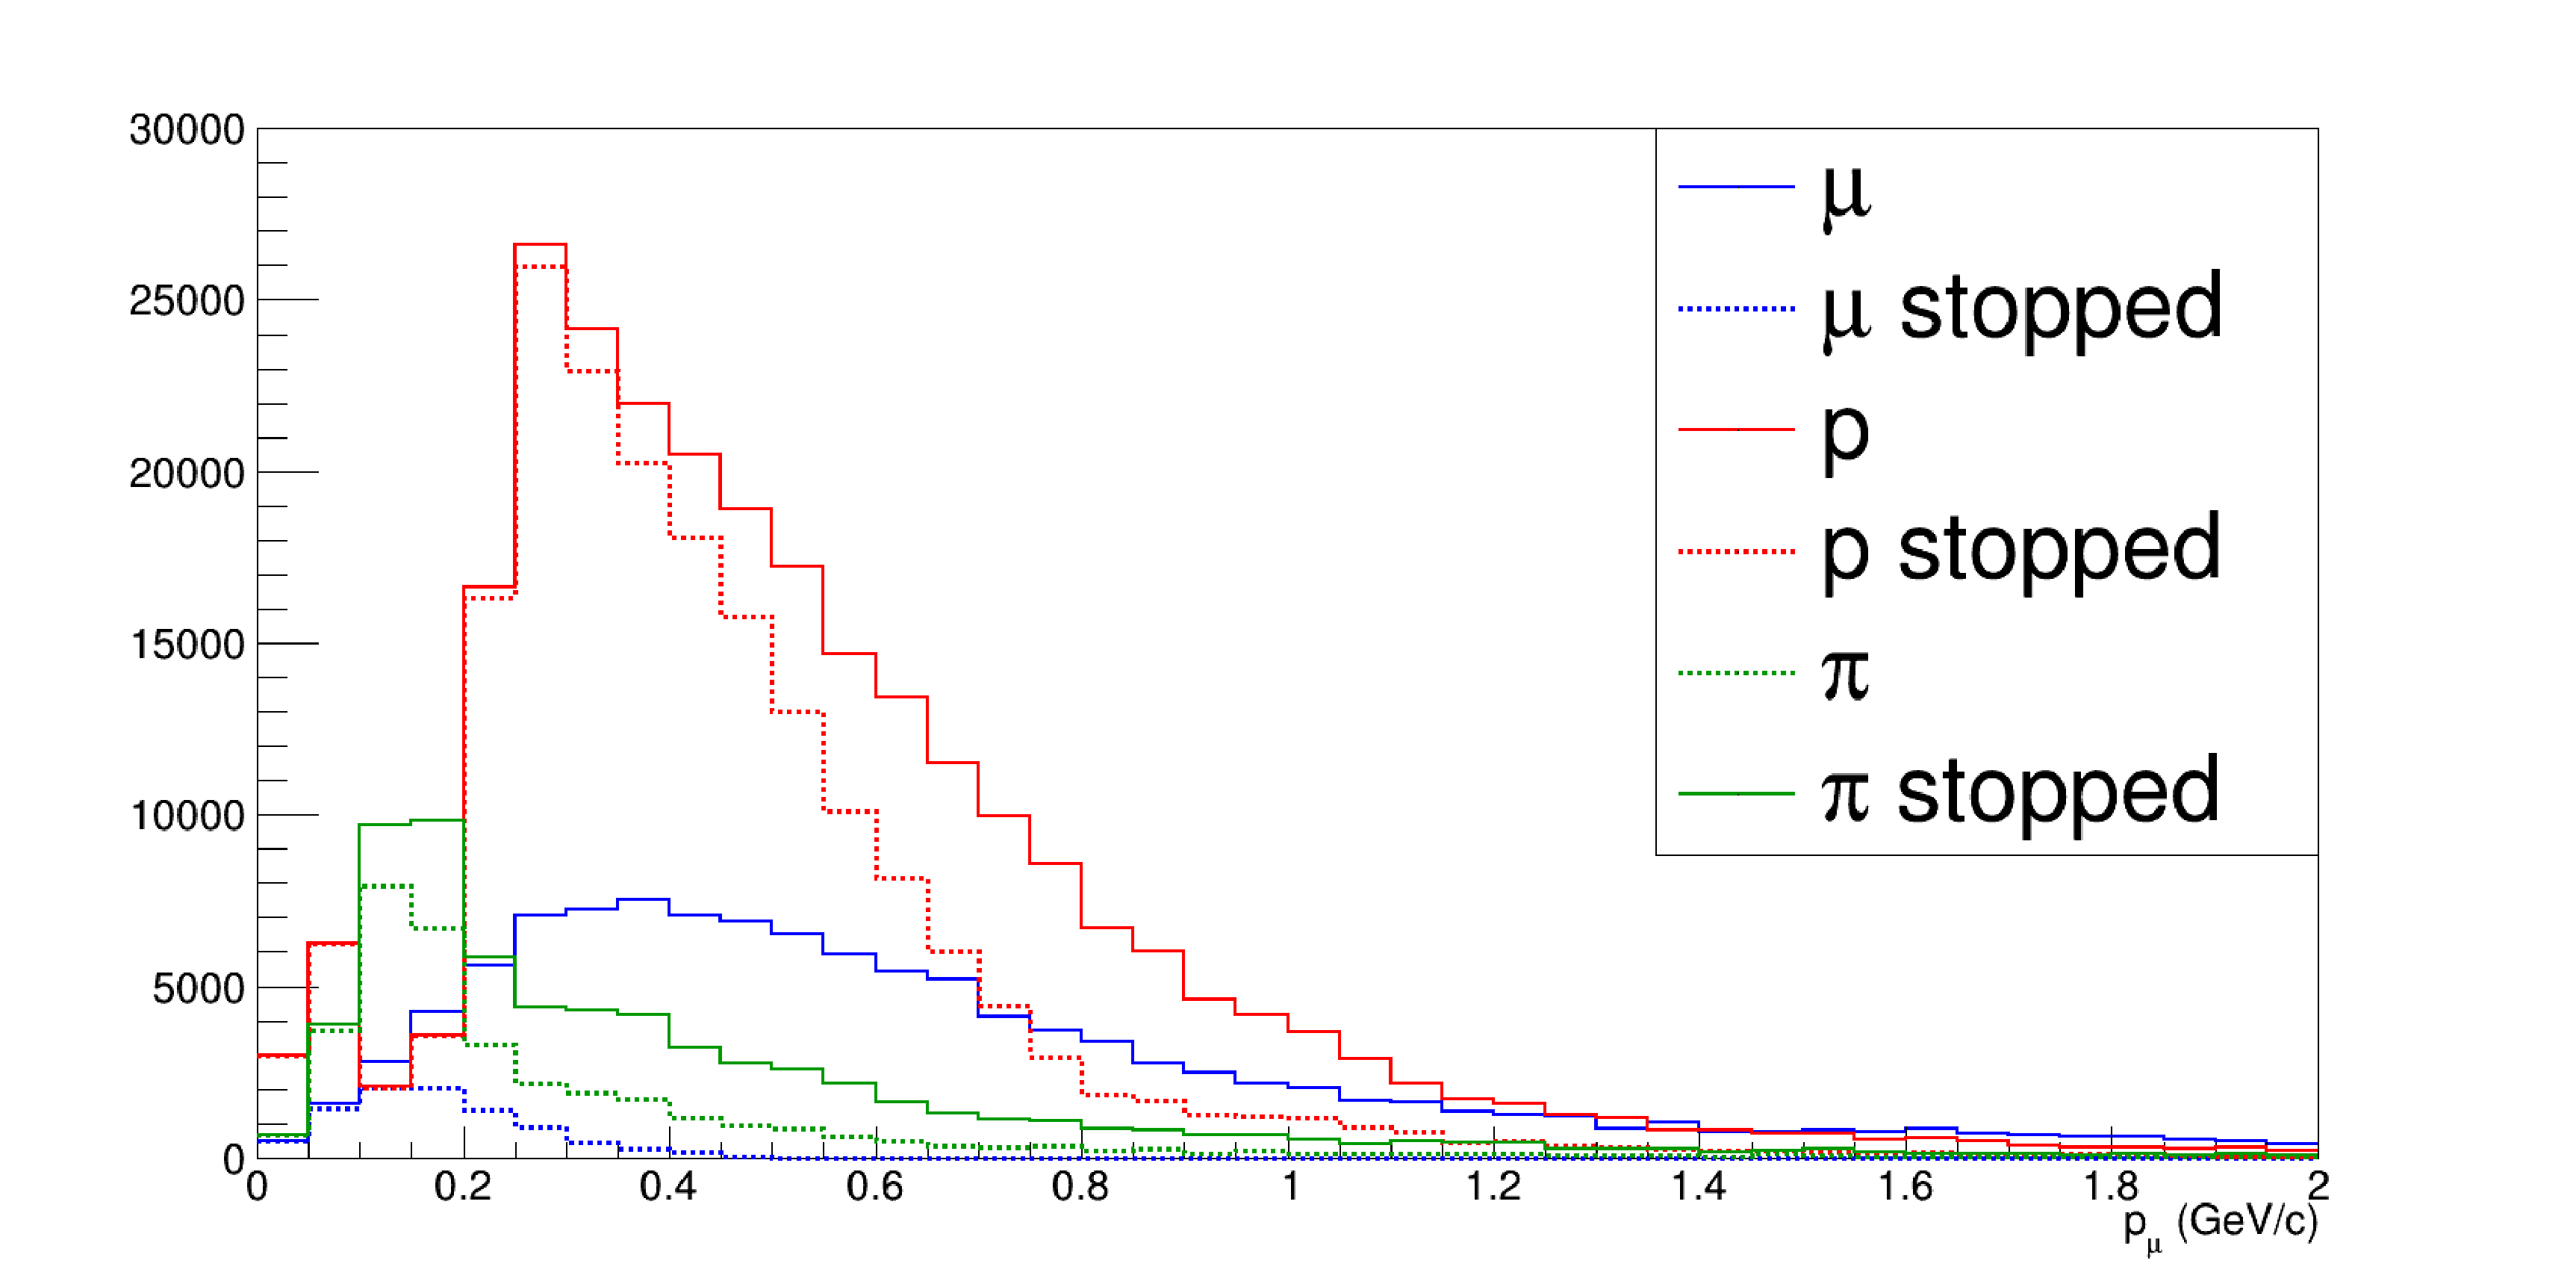
\includegraphics[width=.7\textwidth]{fig/StoppedProportionsMomentum.pdf}
\caption{\label{fig:stoppedproportions} Momentum distribution of true particles in WAGASCI (plain) and corresponding distributions only for particles stopping into the WAGASCI module (dashed).}
\end{figure}

This study is based on an original study done for the ND280 upgrade target, with some modifications. Though the cell size is similar to the WAGASCI configuration presented in Section~\ref{sec:mc_study}, the external dimensions are different ($186.4 \times 60 \times 130~$cm$^{3}$). Whenever the results are presented with this external size and this parameter is likely to impact the result, it will be mentioned.\\
Note that in this section, a simplified reconstruction algorithm presented in Section~\ref{Sec:Reco} is used. The fiducial volume is chosen accordingly as the inner cube of the module which surfaces are distant of $4 \times \text{scintillator space} = 10~$cm from the module external surfaces.\\
The neutrino interactions are simulated using NEUT v5.3.2. The NEUT input neutrino flux is estimated using JnuBeam v13a and assuming the detector to be located at $1.5^{\circ}$ off-axis, as in Section~\ref{sec:mc_study}. Note that the event reconstruction efficiency as a function of true neutrino energy might be changed at 1.5$^{\circ}$, due for example to different $Q^{2}$ distributions. For this reason, one has to note that the reconstruction results might slightly be changed from $2.5^{\circ}$ and $1.5^{\circ}$. To avoid a similar change on the particle-only reconstruction efficiencies, they will be presented as a function of variables that completely characterize the particle kinematic state, \textit{i.e.} its momentum and angle. Figure~\ref{fig:trueinteraction_particle} shows the vertices distributions of the daughter particles of neutrinos interacting one standard WAGASCI water-module. In this section, we will show the detector reconstruction and particle identification in this phase space, both for leptonic and hadronic particles. We will finally show an empty WAGASCI module can highly enhance the ability to constrain the neutrino interaction final state which is critical to reduce the corresponding uncertainties.

\begin{figure}
  \centering
  \begin{subfigure}{.49\textwidth}
    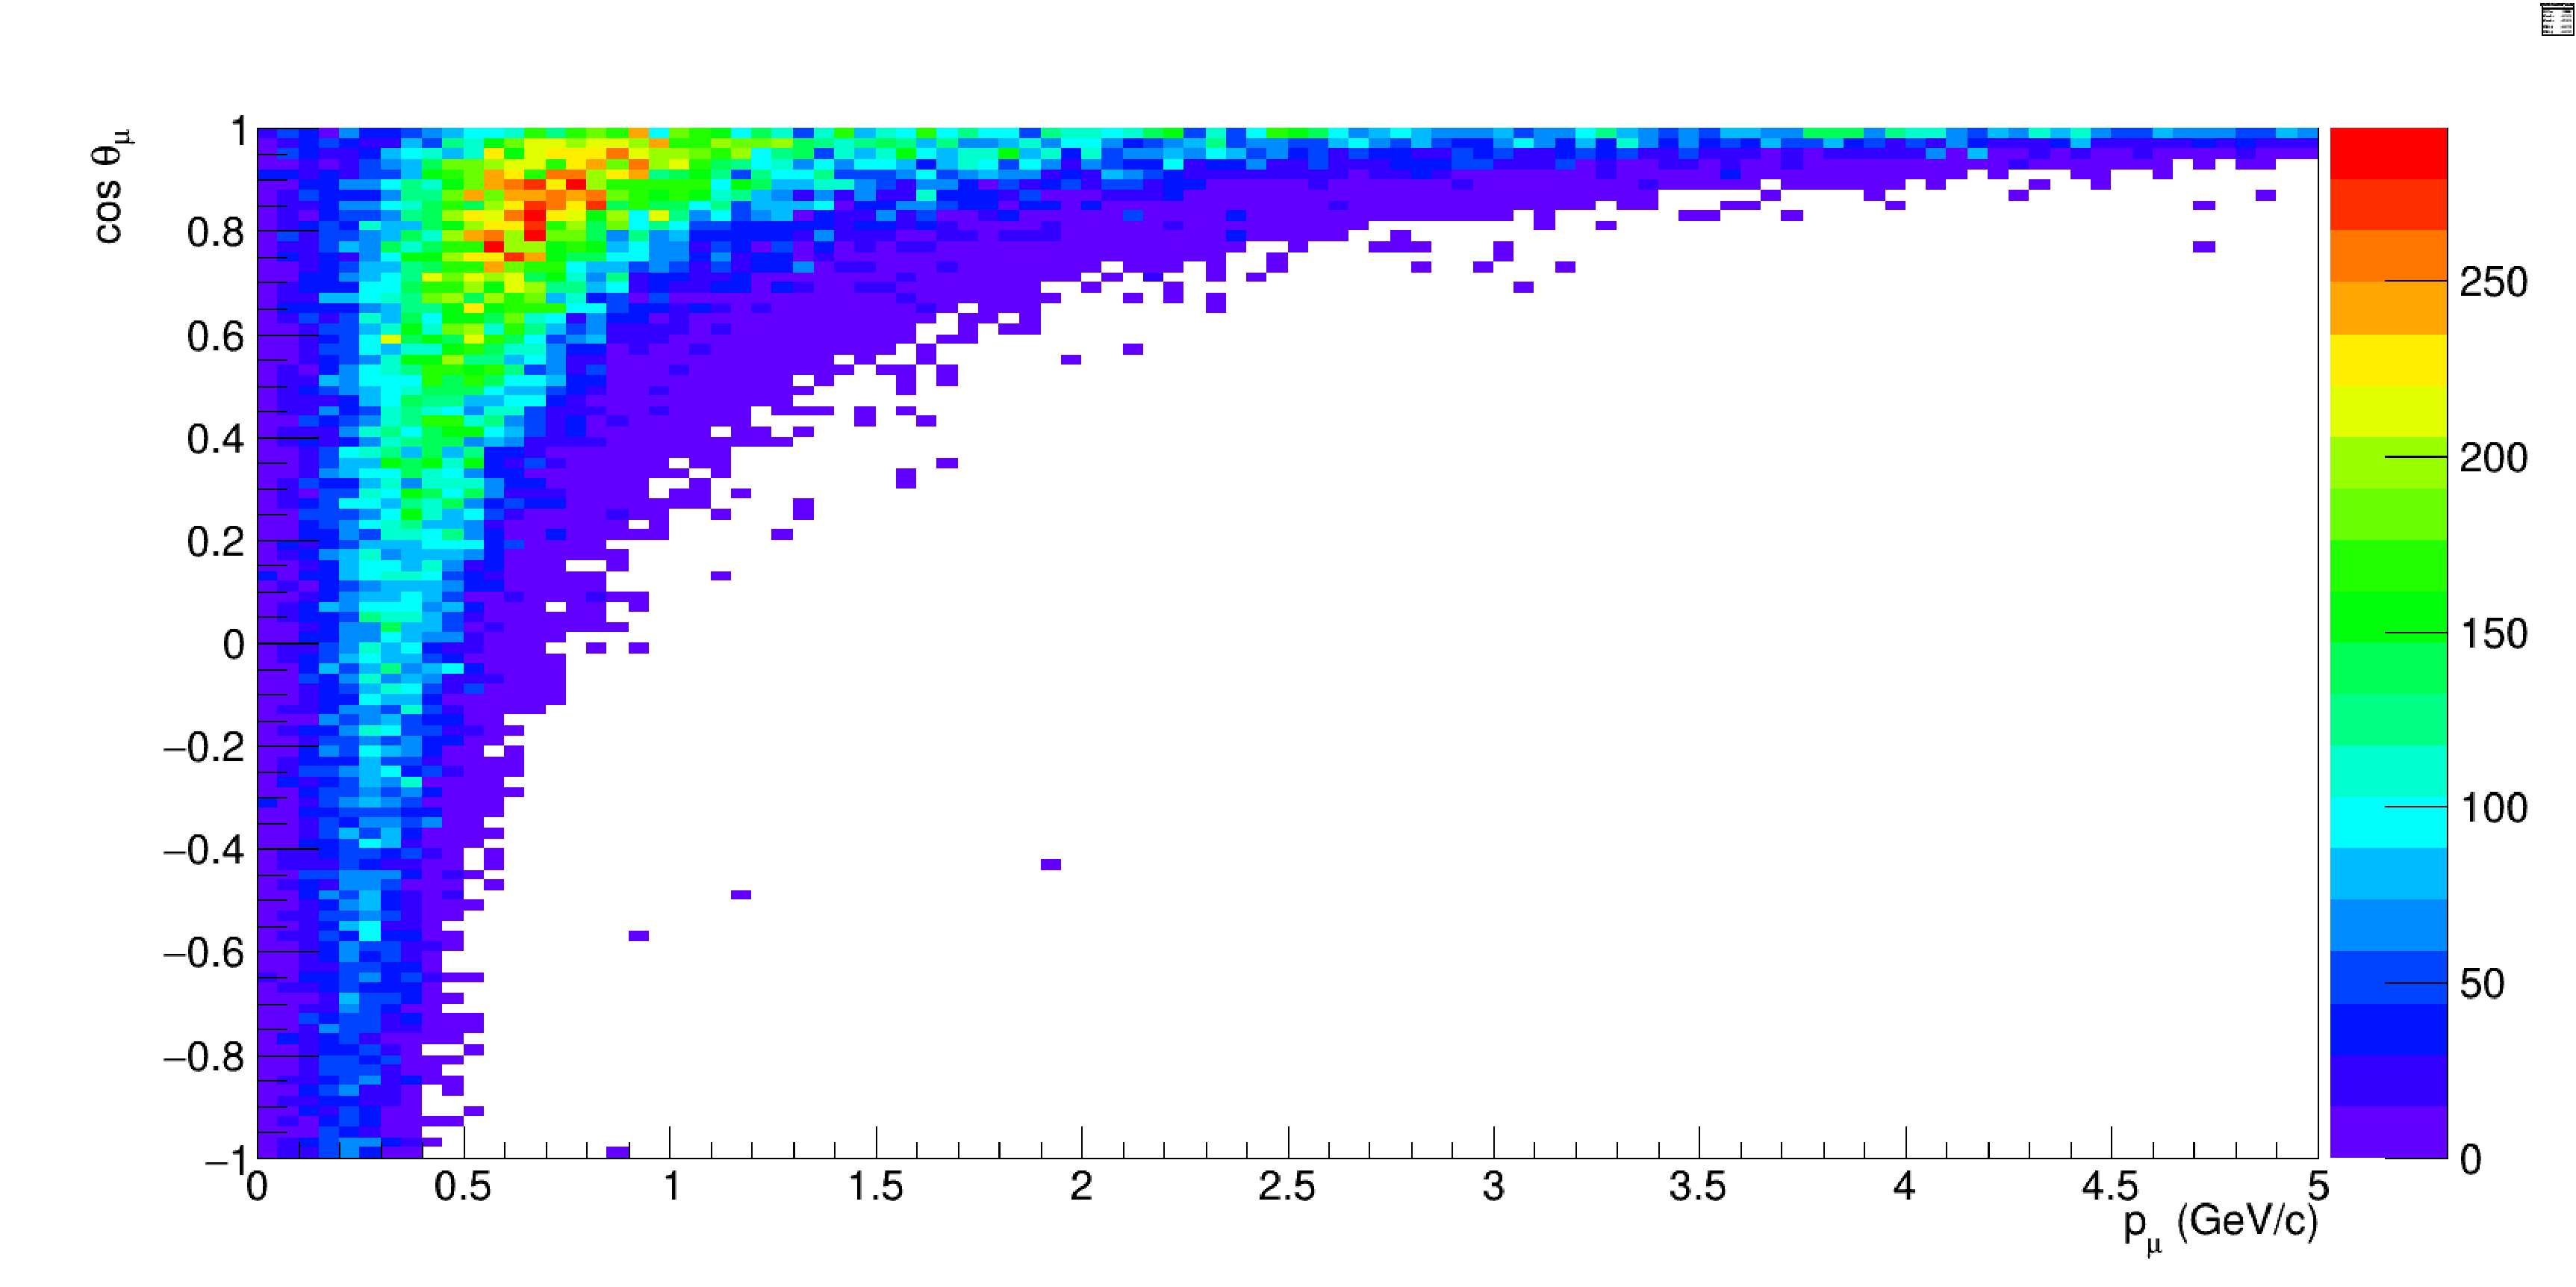
\includegraphics[width=\linewidth]{fig/TrueInteractions_Muon.pdf}
  \end{subfigure}
  \begin{subfigure}{.49\textwidth}
    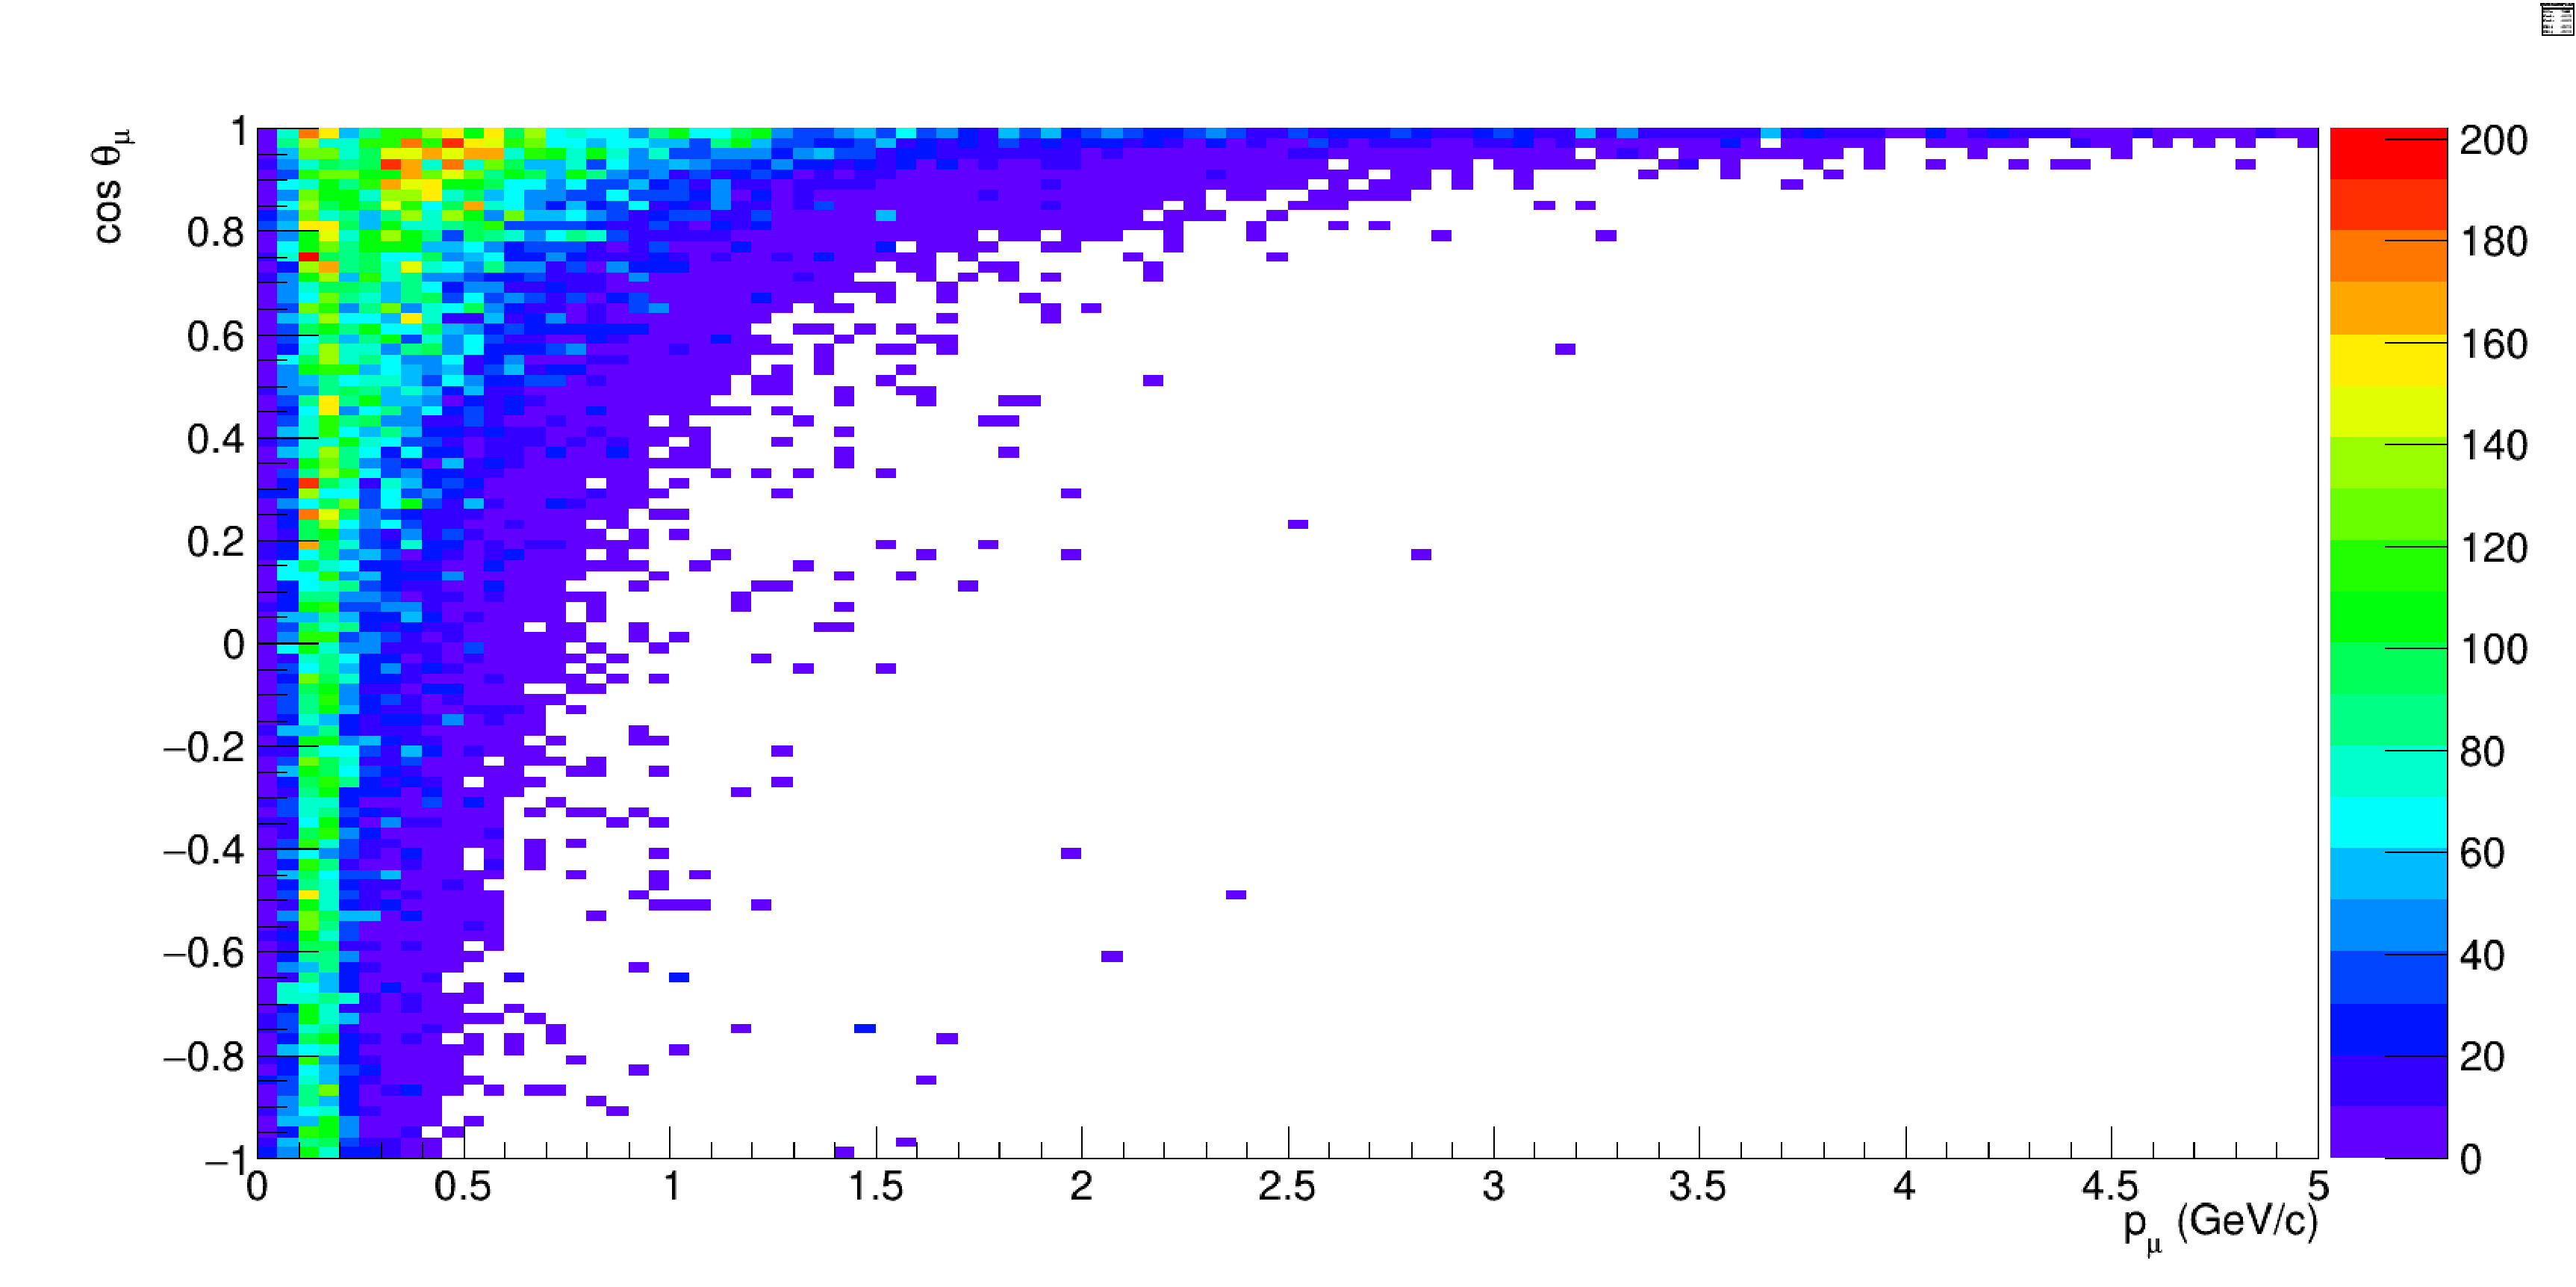
\includegraphics[width=\linewidth]{fig/TrueInteractions_Pion.pdf}
  \end{subfigure}
  \begin{subfigure}{.49\textwidth}
    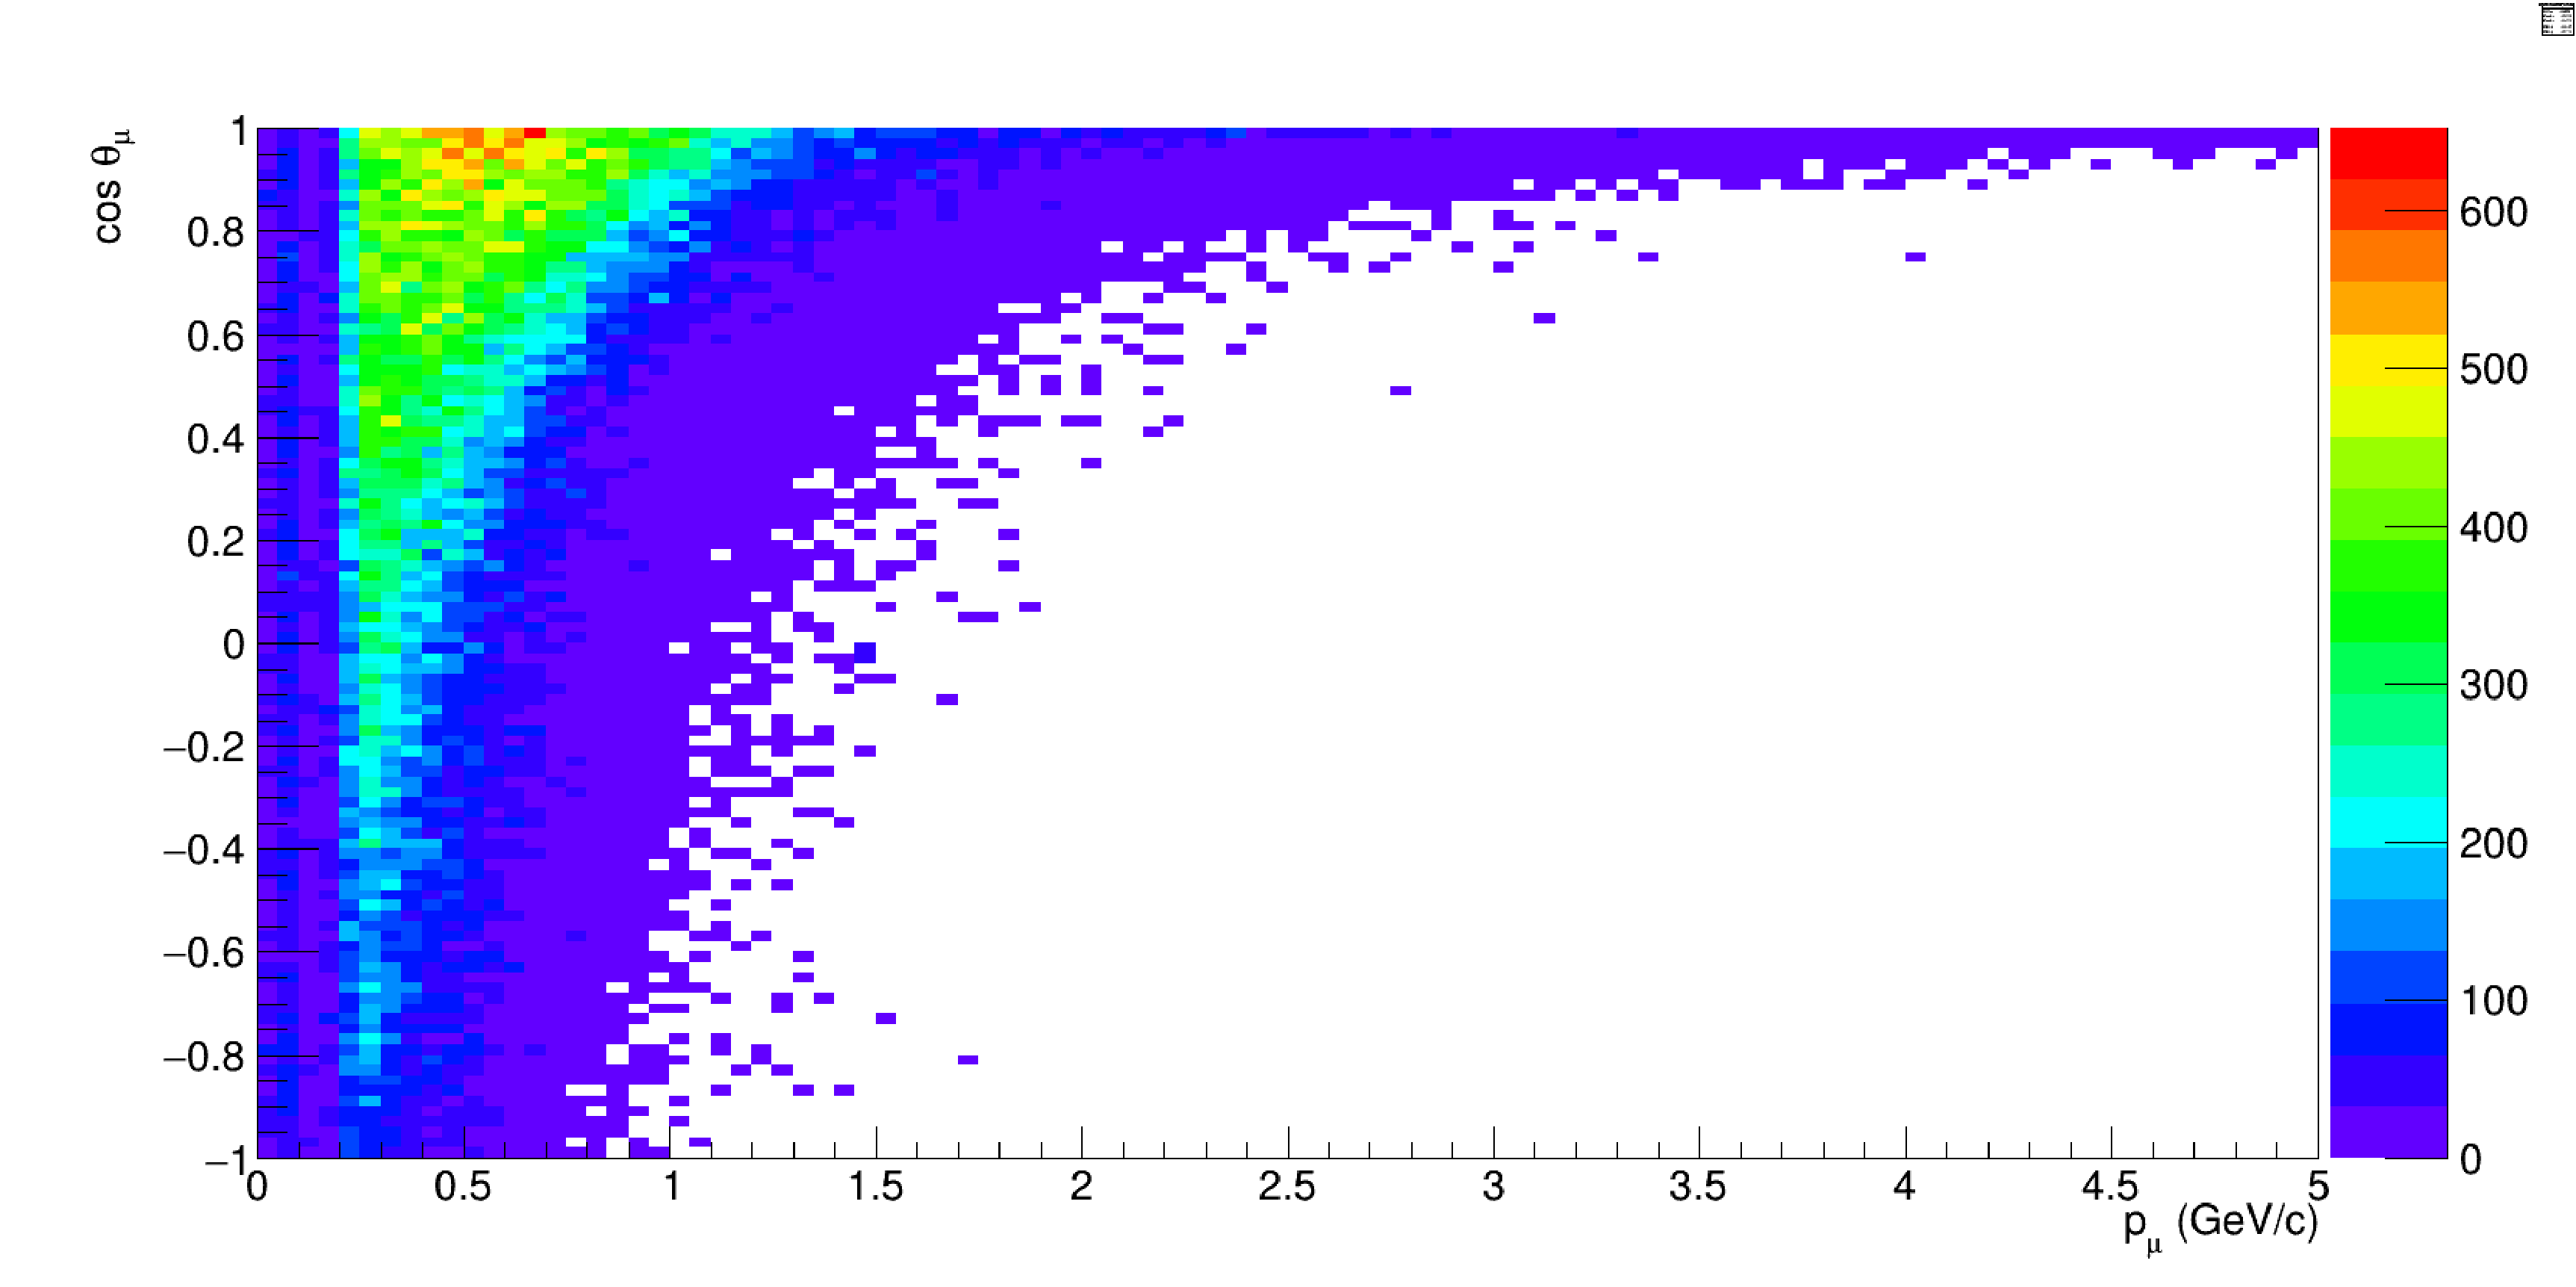
\includegraphics[width=\linewidth]{fig/TrueInteractions_Proton.pdf}
  \end{subfigure}
  \caption{\label{fig:trueinteraction_particle} True number of muons (left), charged pions (right) and protons (bottom) in the two WAGASCI water-module as a function of the particles momenta and angles at $1.5^{\circ}$.}
\end{figure}

\subsection{Reconstruction algorithm}
\label{Sec:Reco}
\subsubsection{Description}
For this section, an ideal ``simulated'' reconstruction is developed. A particle is reconstructed if:
\begin{enumerate}
\item The particle is charged.
\item Lets at least one hit (energy deposit $> 2.5$ photo-electron) in a scintillator.\\
\item The particle enters one TPC and let one hit in the tracker.\\
  Or\\
  \begin{itemize}
  \item The particle should be long enough to be reconstructed by the detector in at least 2 out of 3 views (XZ, YZ, XY). The length criterion requires the particle to let at least 4 hits in the detector. In the ``less favourable case'' of pure longitudinal or tranverse going tracks, it represents a the track length of $L_{track} \geq  4 \times \text{scintillator space} = 10.0~$cm.
  \item In the views where particles pass the length criterion, the particle shall not be superimposed with longer tracks in at least two views. The superposition criterion is estimated with the distance inter-tracks (DIT) which corresponds to the orthogonal distance between two tracks at the ending point of the shortest one (see Figure~\ref{fig:DIT}). For a track 1, the superposition criterion is tested with every longer tracks that starts at the same vertex. Let $\vec{p_{1}}$ the vector of track 1, and $p_{1}^{a}$ its projections in the XZ, YZ and XY planes respectively for i=1,2,3. Note that these are projections in a 2D planes and not on a direction vector. In this case, the relative angle between the track 1 and a longer track 2 (of vector $\vec{p_{2}}$) in a view a is given by:
\begin{equation}
  \cos \theta = \frac{\vec{p_{1}^{a}} \cdot \vec{p_{2}^{a}}}{||\vec{p_{1}^{a}}|| ||\vec{p_{2}^{a}}||} 
\end{equation}
and the distance inter track is given by:
\begin{equation}
  \text{DIT} = ||\vec{p_{1}^{a}}|| \sin \theta
\end{equation}
The DIT should be higher than $4 \times \text{scintillator width}$ for the track 1 to be not superimposed with the track 2 in the view a, which also corresponds to 10.0 cm in the nominal configuration.
  \end{itemize} 
\end{enumerate}
\begin{figure}
  \centering
  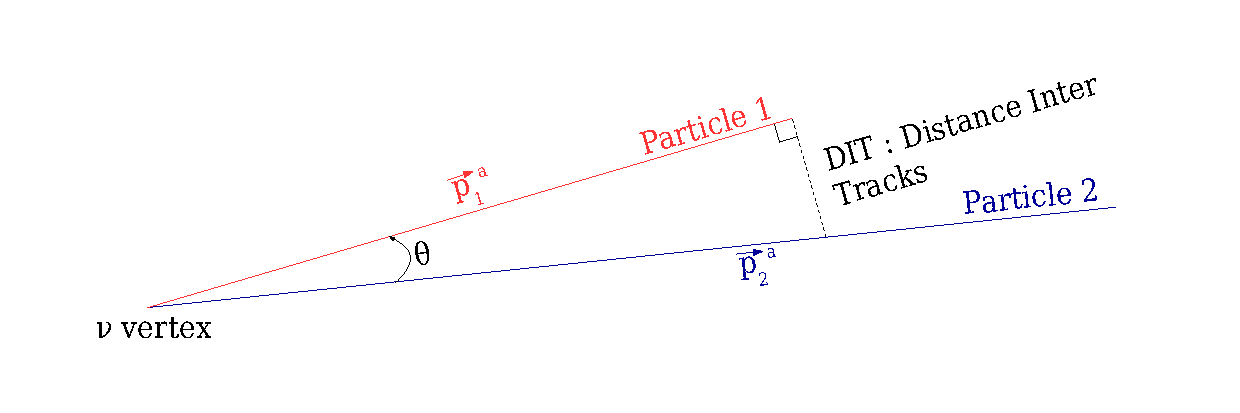
\includegraphics[width=.7\textwidth]{fig/DistanceInterTracks.pdf}
  \caption{\label{fig:DIT} Definition of the distance inter tracks.}
\end{figure}

\subsubsection{Performances}
The particle-only reconstruction efficiencies and the reconstruction threshold in momenta are shown in Table~\ref{tab:reconstructedparticles}. This threshold is defined as the maximal momentum for which the reconstruction efficiency is smaller than $30\%$. The thresholds in muon and pion momenta are $150~$MeV/c. Most of the muons are above this threshold (see Figure~\ref{fig:trueinteraction_particle}) which leads to a $79\%$ reconstruction efficiency. 

\begin{table}[htb]
  \small
  \begin{center}
    \begin{tabular}{|c|c|c|c|}
      \hline
      \hline
      & $\mu$ & $\pi$ & p \\
      \hline
      Reconstruction Efficiency & 79\% & 52\% & 26\% \\
%      Purity & 56\% & 14\% & 31\% \\
      Momentum threshold & 150 MeV/c & 150 MeV/c & 550 MeV/c \\
      \hline
      \hline
    \end{tabular}
    \caption{\label{tab:reconstructedparticles} Reconstruction efficiency and momentum threshold for muons, pions and protons. The threshold is defined as the maximal momentum for which particles have a reconstruction efficiency smaller than $30\%$.}
  \end{center}
\end{table}
 The lower pion and proton efficiencies (respectively $52\%$ and $26\%$) are due to lower efficiencies for similar momenta than muons, coming from strong interactions as shown on Figures~\ref{fig:efficiency_particle}. Efficiencies of each particle type tend to decrease in the backward region due to particle lower momenta. However, for a fixed momentum value, the reconstruction efficiency is almost uniform which confirms the ability of the WAGASCI detector to reconstruct high angle tracks. 
\begin{figure}
  \centering
    \begin{subfigure}{.49\textwidth}
    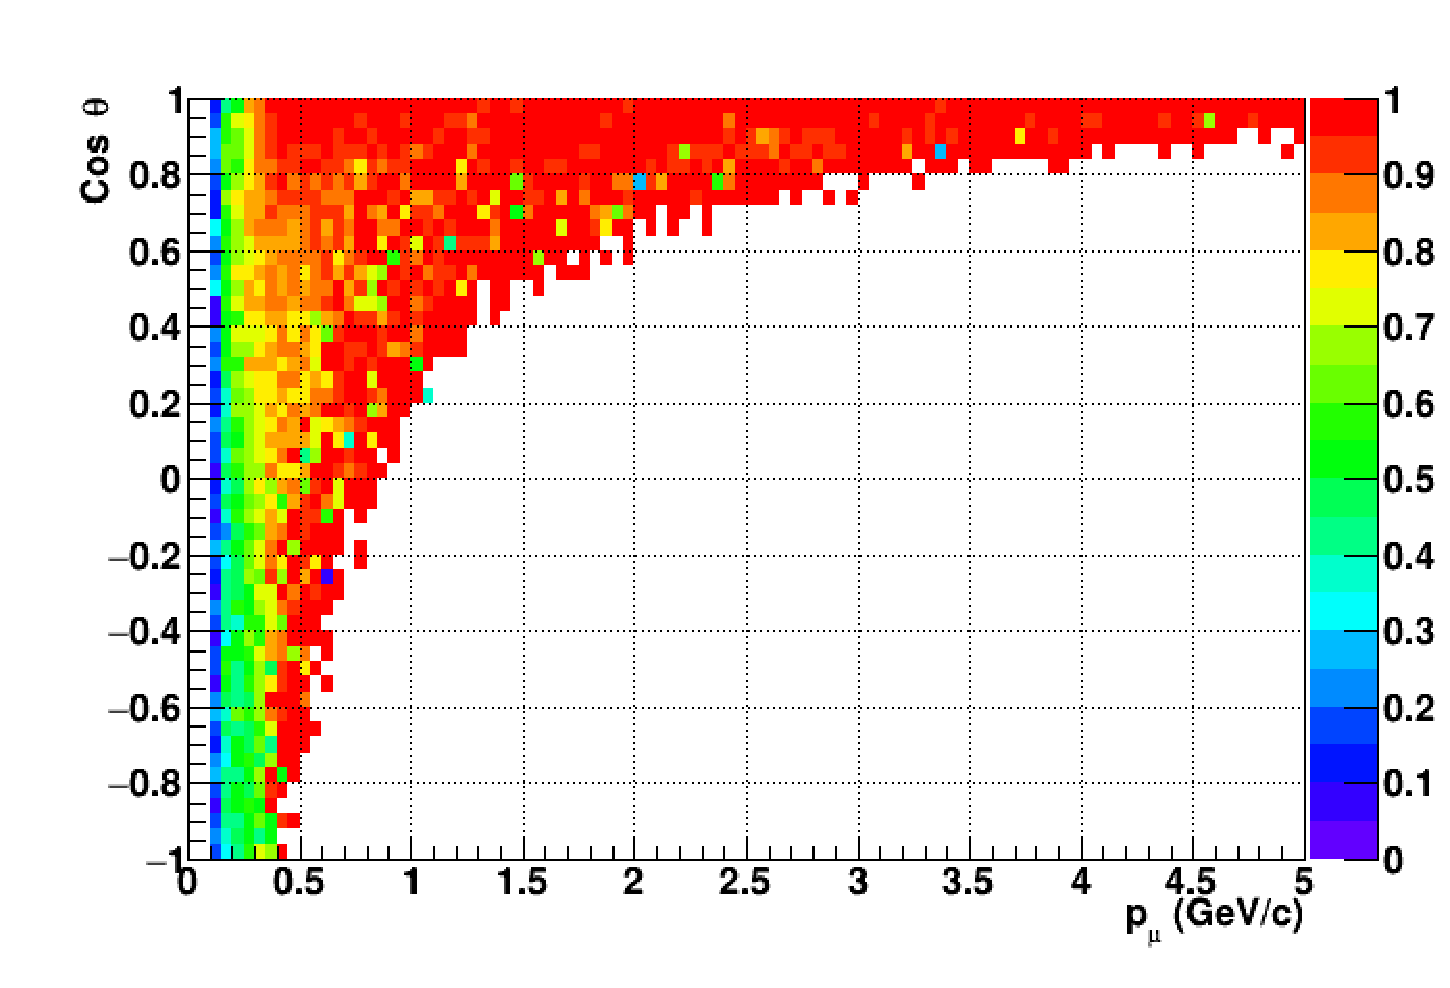
\includegraphics[width=\linewidth]{fig/Efficiency_Muon.pdf}
  \end{subfigure}
    \begin{subfigure}{.49\textwidth}
    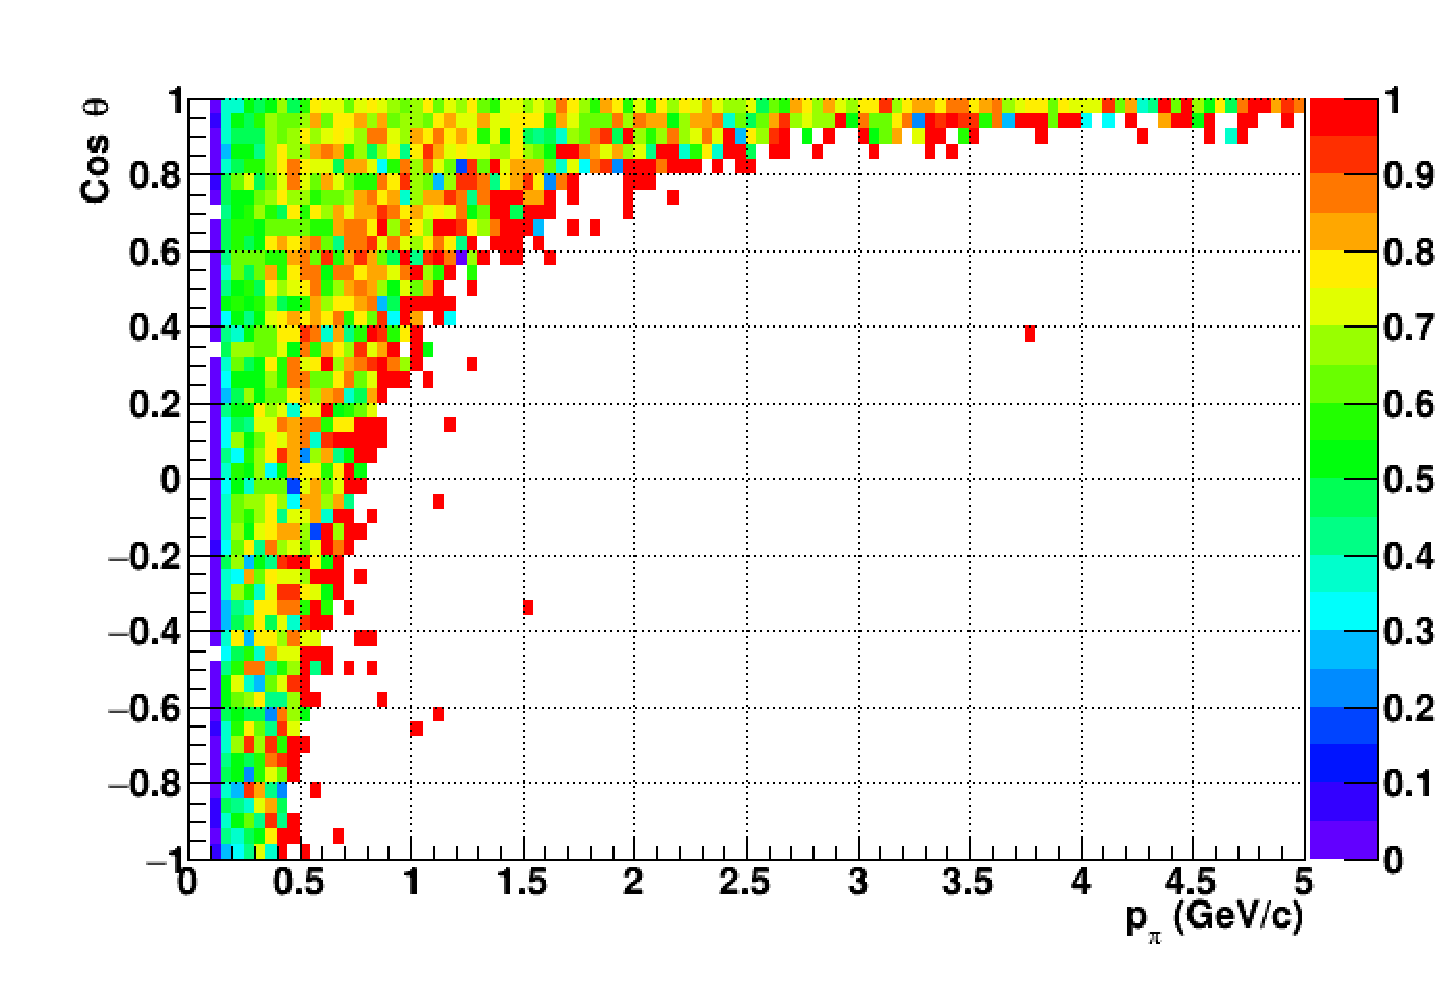
\includegraphics[width=\linewidth]{fig/Efficiency_Pion.pdf}
  \end{subfigure}
    \begin{subfigure}{.49\textwidth}
    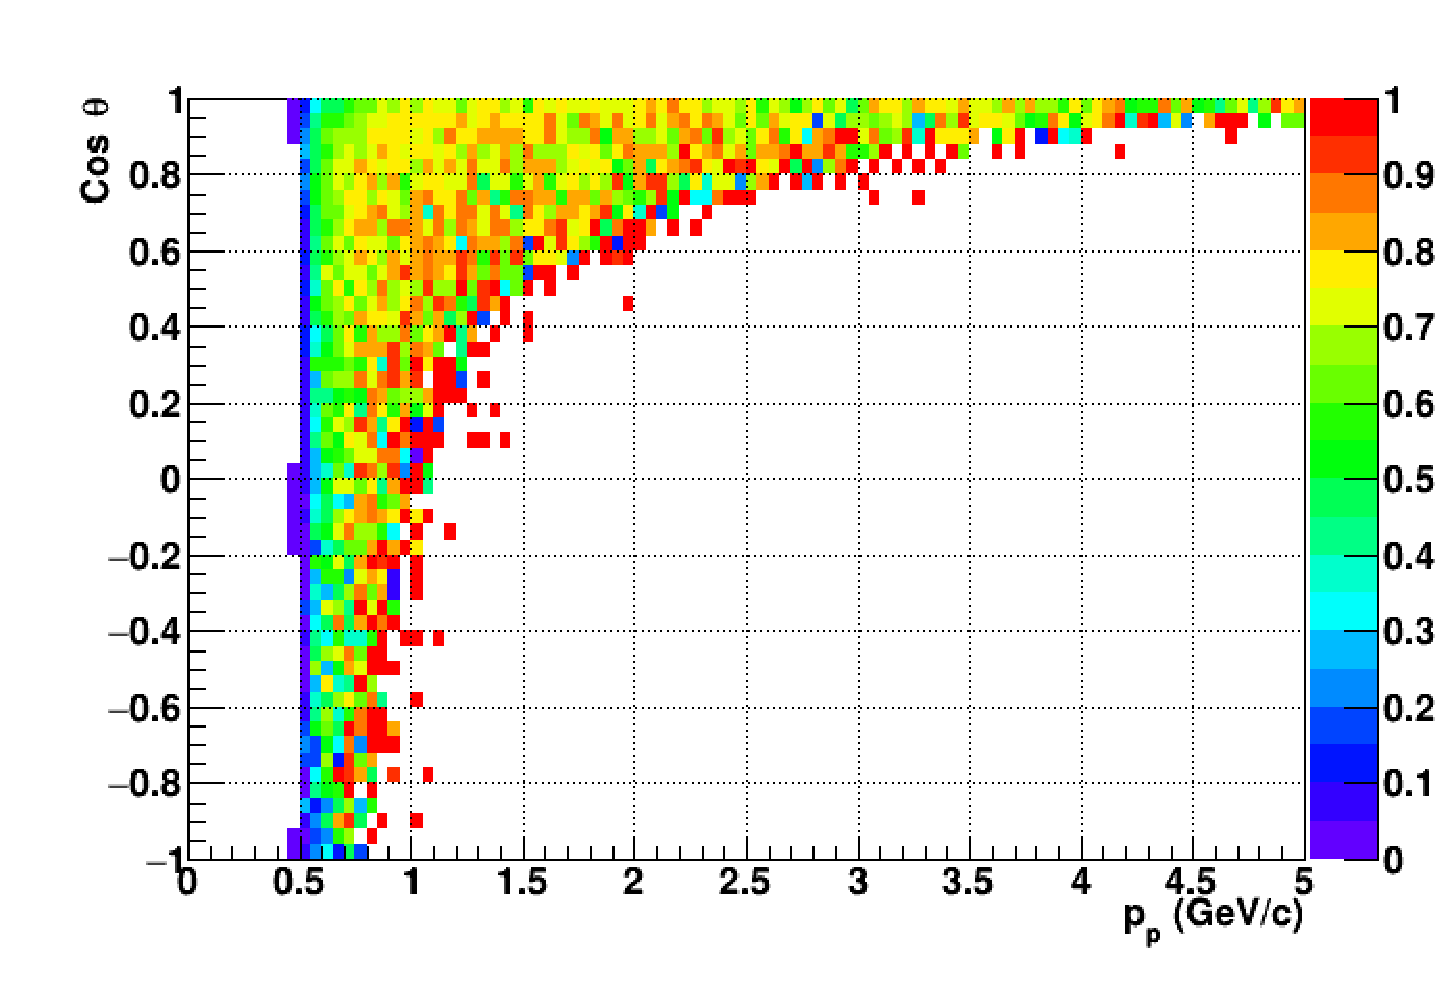
\includegraphics[width=\linewidth]{fig/Efficiency_Proton.pdf}
  \end{subfigure}
  \caption{\label{fig:efficiency_particle} Reconstruction efficiency of muons (left), charged pions (right) and protons (bottom) in the WAGASCI water-module as a function of the particles momenta and angles.}
\end{figure}


The reconstruction is thereafter tested on neutrino events. Table~\ref{tab:reconstructedinteractions} summarizes the number of reconstructed events and efficiencies for each interaction type. As expected from the high muon reconstruction efficiency, the charged current interactions have reconstruction efficiencies $\geq 85\%$.
\begin{table}[htb]
  \small
  \begin{center}
    \begin{tabular}{|c|c|c|c|c|c|}
      \hline
      \hline
      & CC0$\pi$ & CC1$\pi$ & CCOthers & NC & All \\
      \hline
      Reconstruction efficiency & 85\% & 87\% & 91\% & 22\% & 68\% \\
      \hline
      \hline
    \end{tabular}
    \caption{\label{tab:reconstructedinteractions} Number of true interactions reconstructed. The purity and reconstruction efficiency of each true interaction is also shown.}
  \end{center}
\end{table}

The reconstruction efficiencies as a function of the neutrino energy and muon kinematics are respectively shown on Figure~\ref{fig:efficiency_enu} and \ref{fig:efficiency_muonkinematics}.
\begin{figure}
  \centering
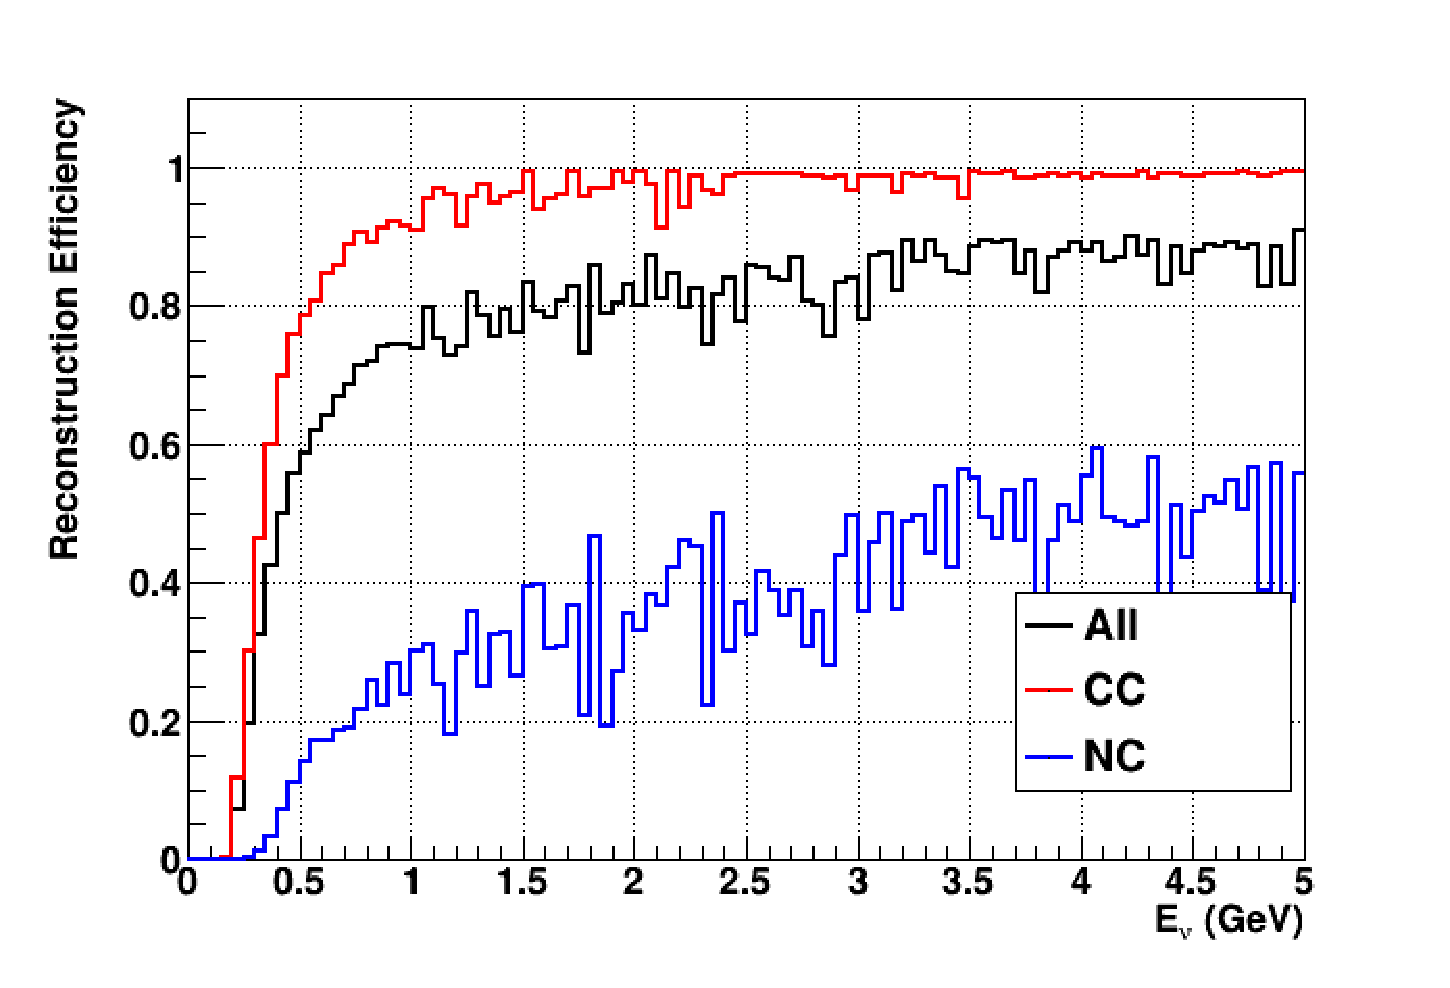
\includegraphics[width=.7\textwidth]{fig/Efficiency_Enu.pdf}
  \caption{\label{fig:efficiency_enu} Reconstruction efficiency of all neutrino (black), CC (red) and NC (blue) interactions in the WAGASCI water-module as a function of the neutrino energy.}
\end{figure}
\begin{figure}
  \centering
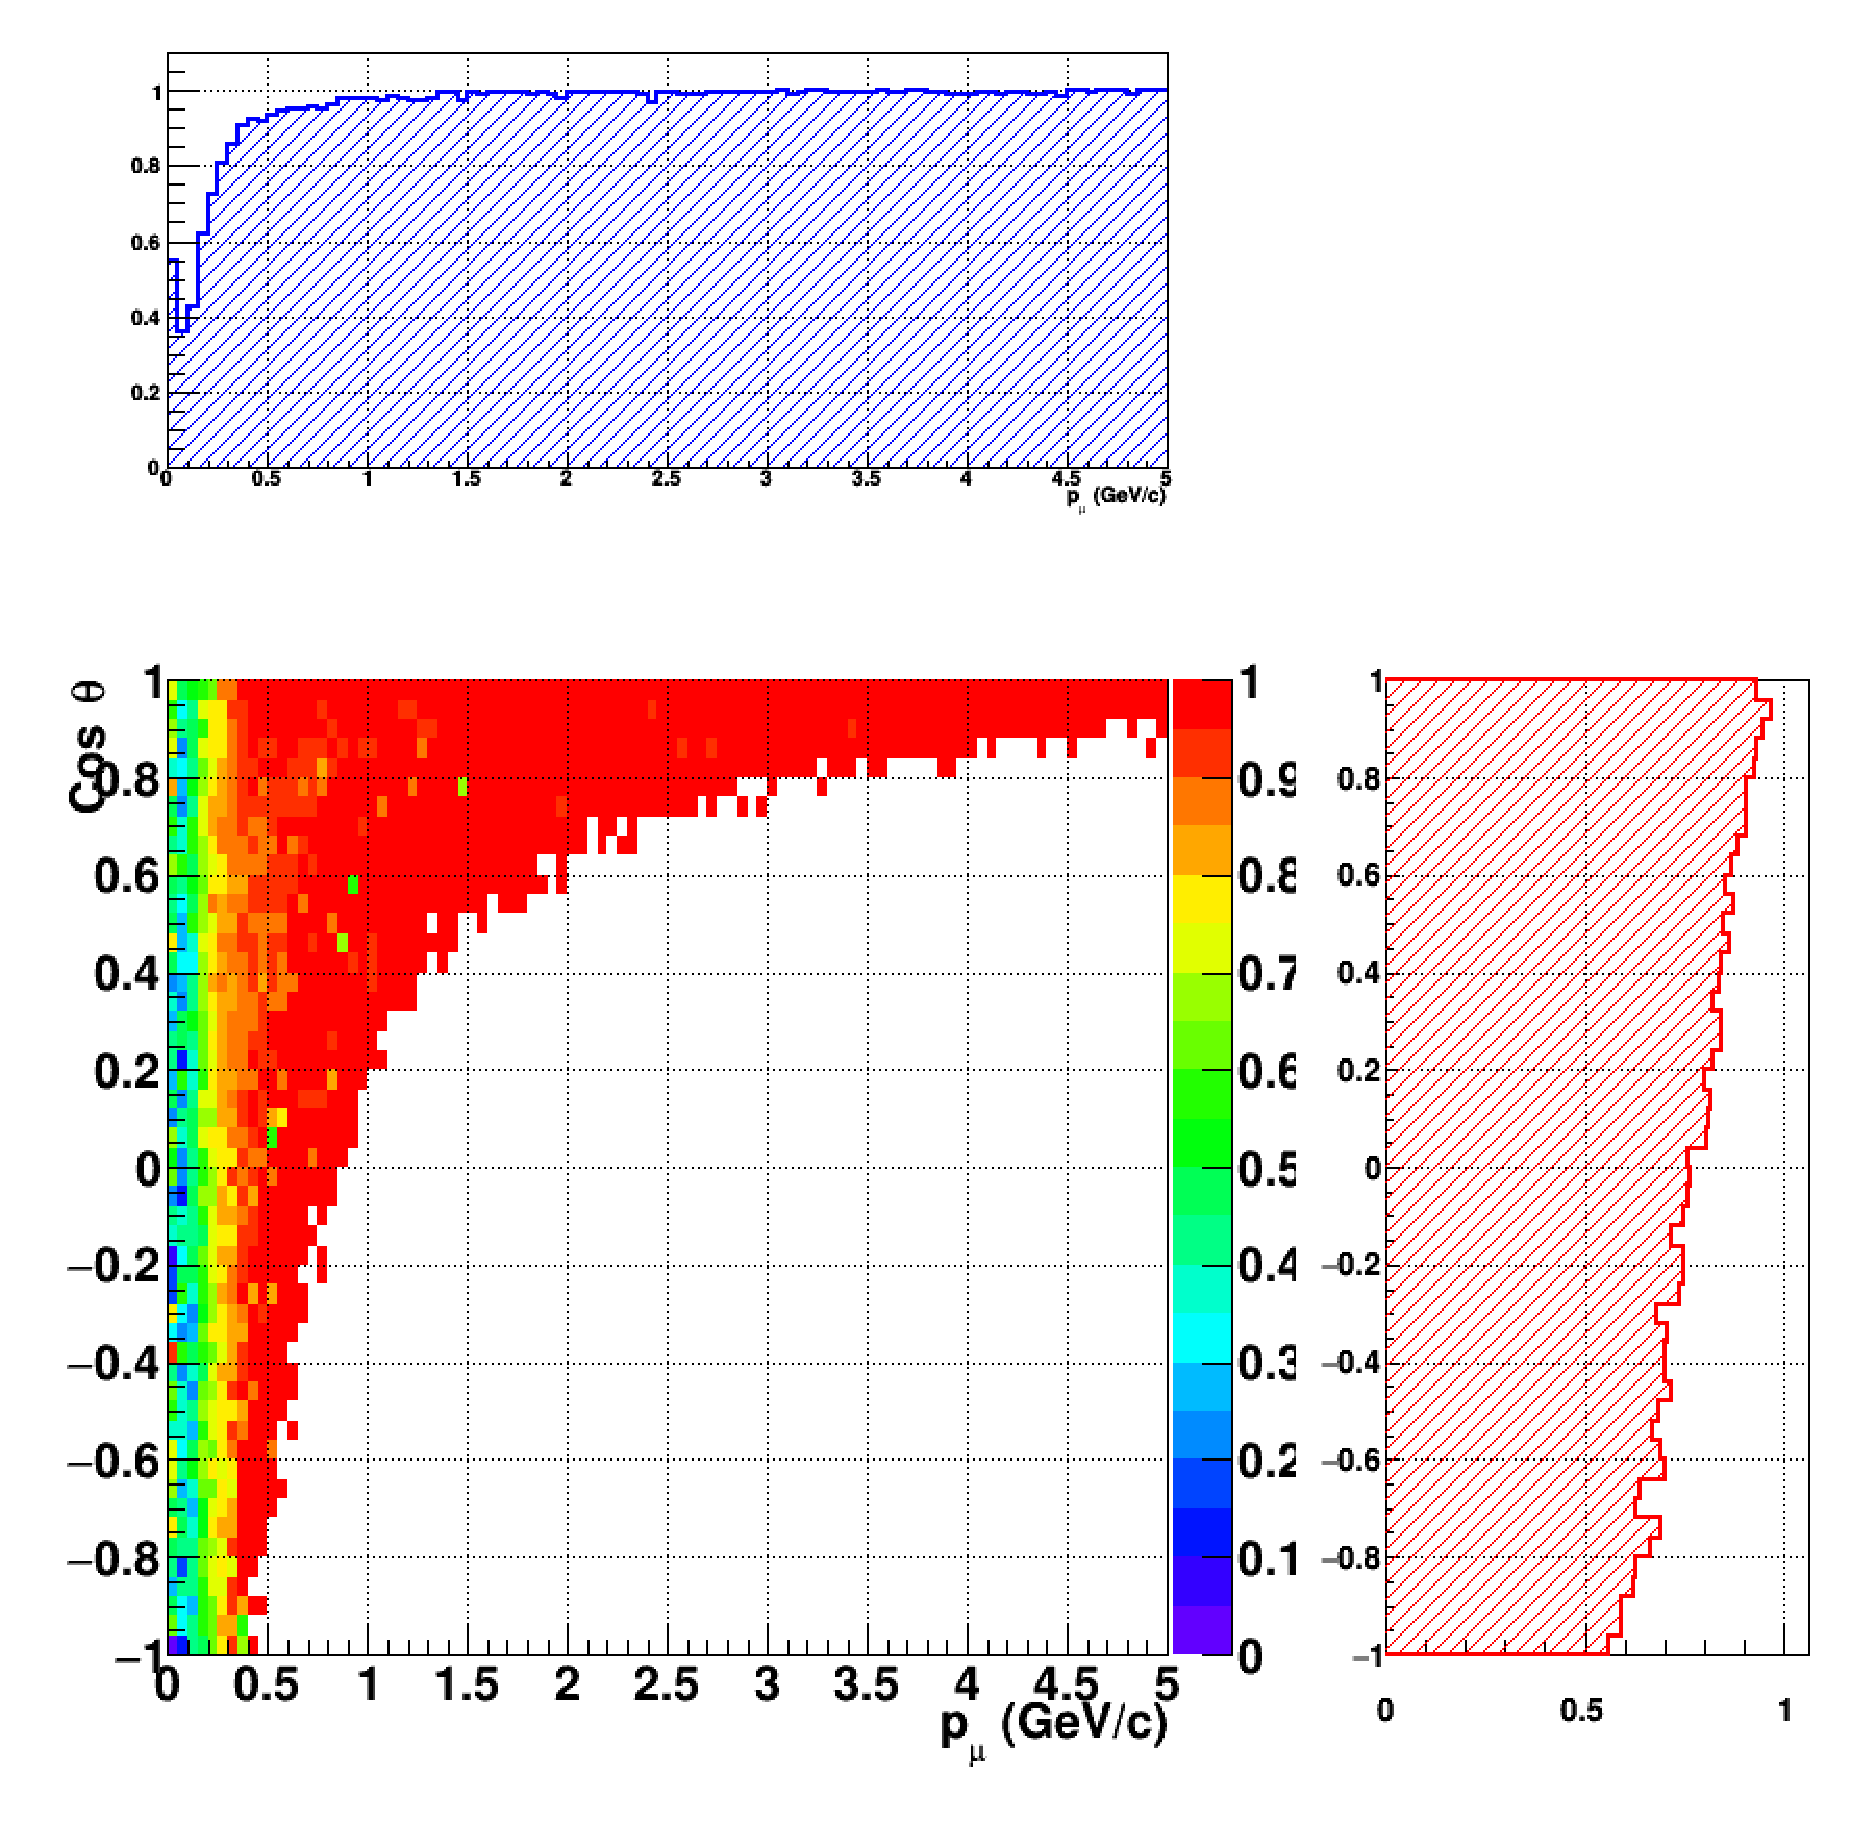
\includegraphics[width=.7\textwidth]{fig/Efficiency_MuonKinematics.pdf}
  \caption{\label{fig:efficiency_muonkinematics} Reconstruction efficiency of CC interactions in the WAGASCI water-module as a function of the muon kinematic variables (momentum and angle).}
\end{figure}
\clearpage

Note that a Particle Identification Algorithm has been also developed. It is based on the charge deposition of the particles in the scintillator, of the detection of a decay-electron. However, this information highly depends on the number of scintillator hit by a particle, which creates an important difference between a real WAGASCI module and the one used for the ND280-upgrade simulation. For this reason, the corresponding results will not be detailed here, but can be found in~\cite{ND280Upgrade}.

\subsection{Background substraction: the water-out module}
In the nominal configuration, $20\%$ of the neutrino interactions occurs on scintillators (C$_{8}$H$_{8}$). This background should be removed in order to measure the neutrino interaction on the same target as Super-K, which suppress the differences in cross-section models. For this purpose, we propose to use a water-out module, where the water is replaced by air. The detector is therefore fully active and has a $3~$mm spatial resolution (scintillator thickness) which create and ideal detector to reconstruct and identify hadrons, and study np-nh interactions. The counter-part is the difference in particle energy deposition between the water and this water-out module that will need to be corrected for. In this section, we present the capabilities of such a module, and the impact it can have on cross-section measurements for the neutrino community in genral and T2K in particular.\\
The same reconstruction and selection as the water-in module is applied. Figure~\ref{fig:reconstructionefficiencyparticle_mometum} shows the comparison between the water-in and the water-out reconstruction efficiencies for muon, pions and protons. $90\%$ of the muons and $87\%$ of the pions are reconstructed, while $70\%$ of the protons are even reconstructed. It allows to low down the proton threshold to 250~MeV/c (see Table~\ref{tab:reconstructedparticles_empty}).     
%Number of interactions: true, reconstructed, selected.
%Efficiency particle per particle.
%Efficiency interaction per interaction
\begin{figure}
  \centering
    \begin{subfigure}{.49\textwidth}
      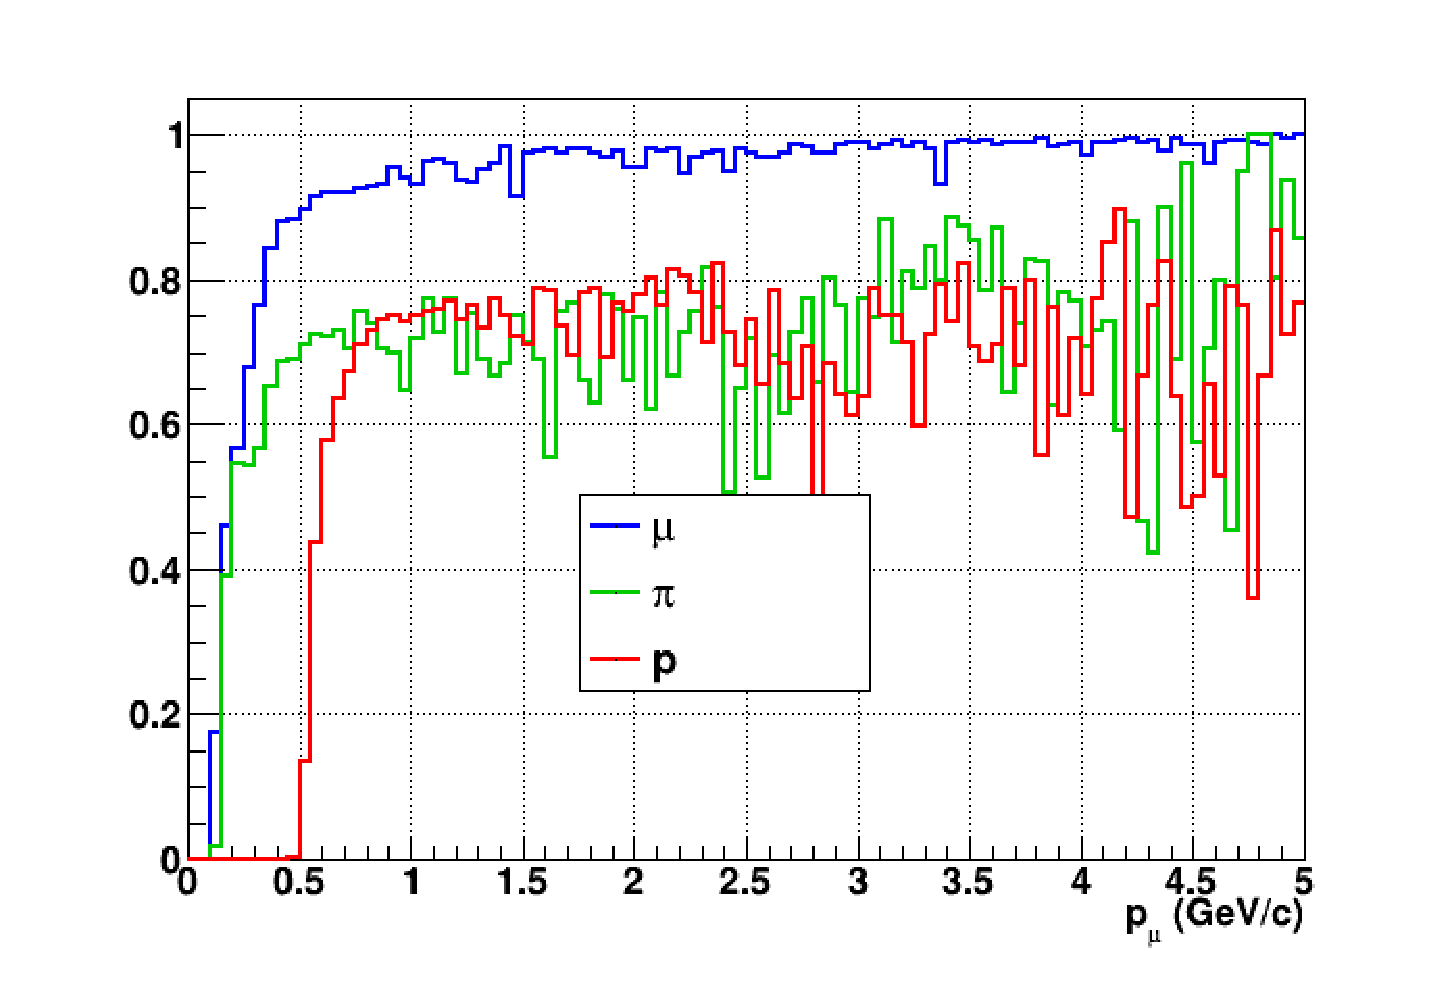
\includegraphics[width=\linewidth]{fig/EfficiencyParticles_Momentum.pdf}
    \end{subfigure}
    \begin{subfigure}{.49\textwidth}
      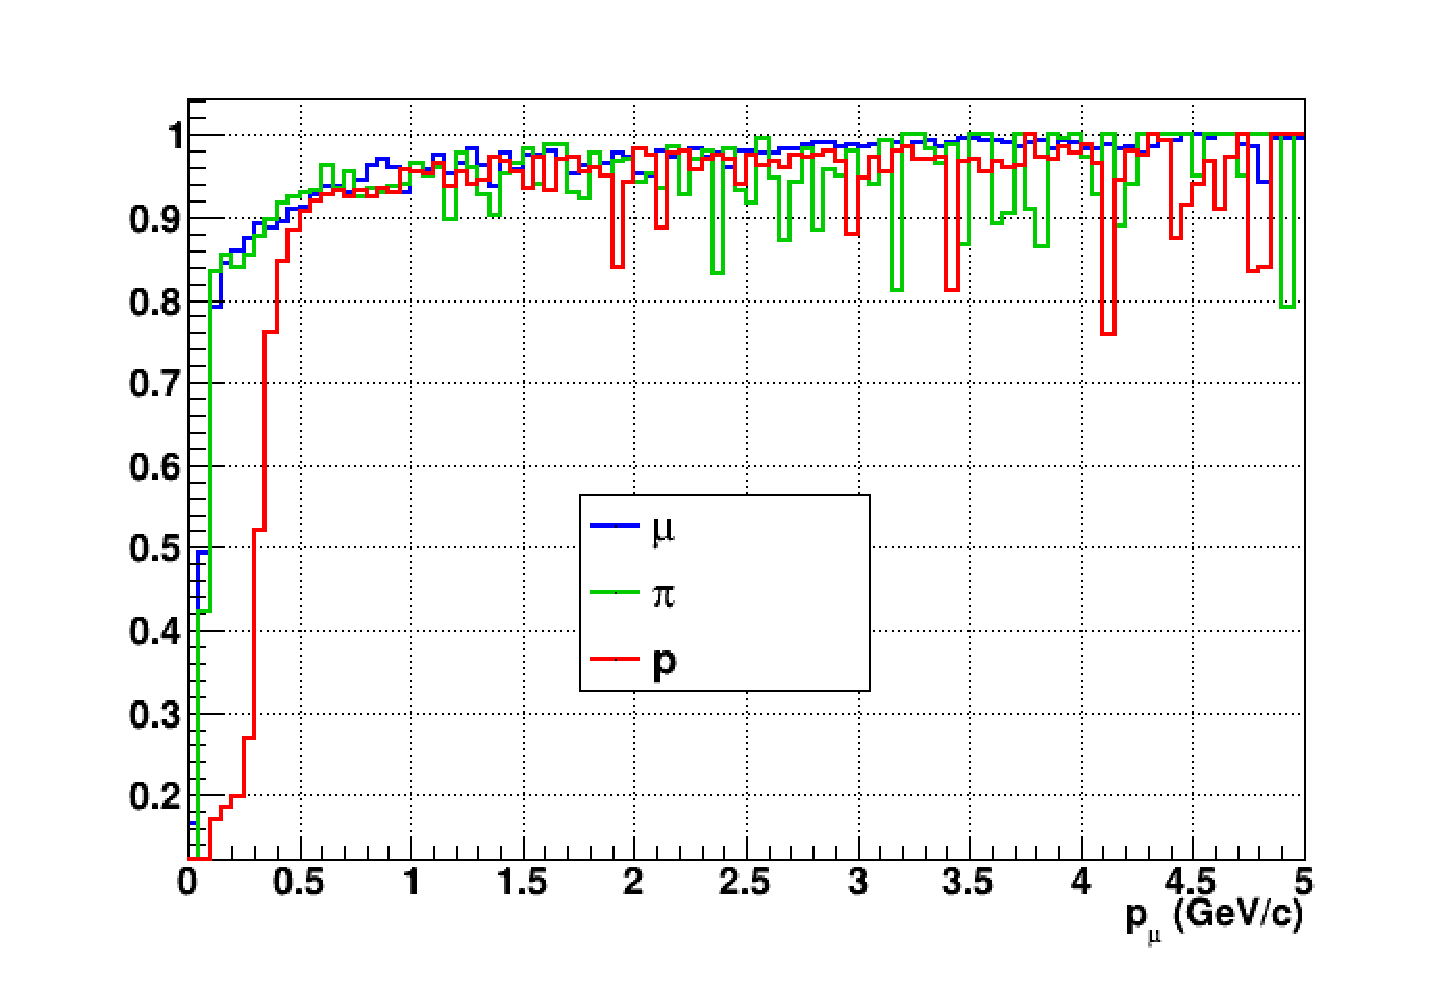
\includegraphics[width=\linewidth]{fig/EfficiencyParticles_Momentum_Empty.pdf}
    \end{subfigure}
  \caption{\label{fig:reconstructionefficiencyparticle_mometum} Reconstruction efficiency for muons, pions and protons in the water-in (left) and water-out (right) modules.}
\end{figure}

\begin{table}[htb]
  \small
  \begin{center}
    \begin{tabular}{|c|c|c|c|}
      \hline
      \hline
      & $\mu$ & $\pi$ & p \\
      \hline
      Reconstruction Efficiency & 90\% & 87\% & 70\% \\
 %     Reconstruction Purity & 37\% & 13\% & 49\% \\
      Momentum threshold & 50 MeV/c & 50 MeV/c & 250 MeV/c  \\
      \hline
      \hline 
    \end{tabular}
    \caption{\label{tab:reconstructedparticles_empty} Reconstruction efficiency, proportions of $\mu$-like and non $\mu$-like and momentum threshold for muons, pions and protons in the empty module. The threshold is defined as the maximal momentum for which particles have a reconstruction efficiency smaller than $20\%$.}
  \end{center}
\end{table}
As a consequence of tracking even low momenta particle, the reconstruction efficiency is uniform and almost maximal on the entire $\cos \theta_{\mu}$ phase space, as shown on Figure~\ref{fig:efficiency_muonkinematics_empty}. Since the fiducial mass represents 0.25~tons, the total number of events is divided by a factor of 3 compared to the water-in module. The water-out module offers interesting possibilities to study np-nh interaction since $70\%$ of the protons are reconstructed. In the future, a possible separation as a function of the number of proton track will be studied. Morevover, we are currenly pursuing the use of single and double transverse variables (cite Xianguo) to open new possibilities for separating np-nh from Final State Interactions, or for isolating the interactions on hydrogen from interactions on carbon in this module. 
%CHekc the proportions of stopped in 1cm3 cell and water-out

\begin{figure}
  \centering
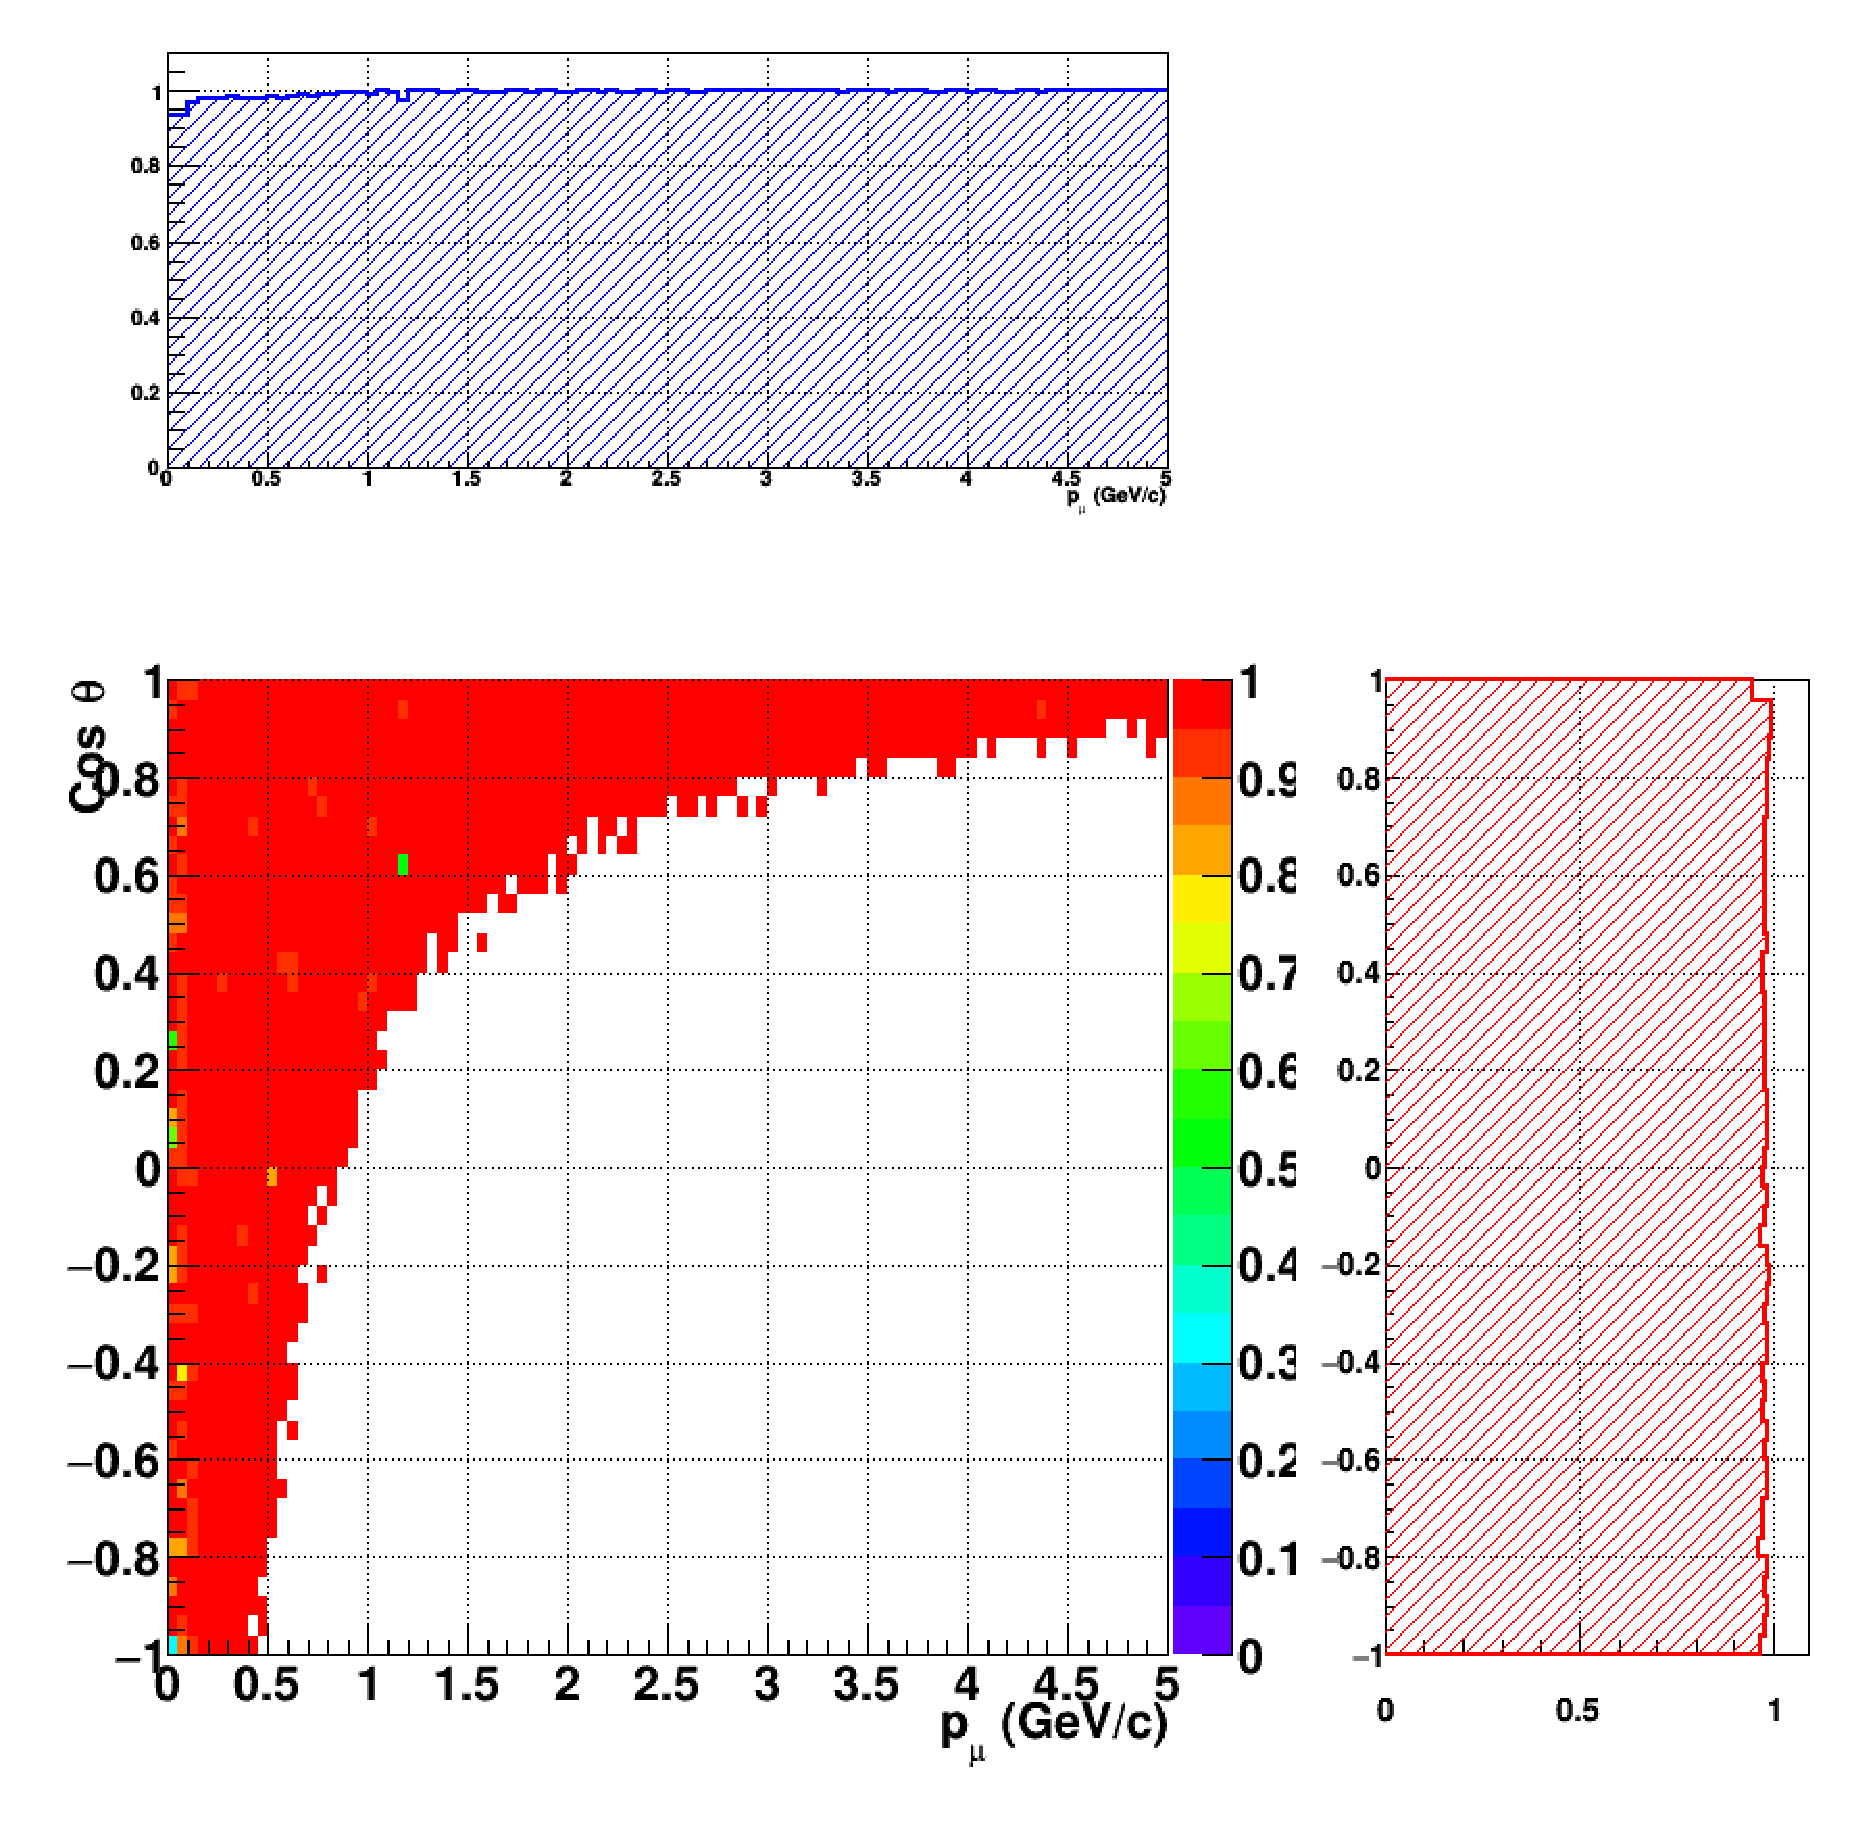
\includegraphics[width=.7\textwidth]{fig/Efficiency_MuonKinematics_Empty.pdf}
  \caption{\label{fig:efficiency_muonkinematics_empty} Reconstruction efficiency of CC interactions in the WAGASCI empty module as a function of the muon kinematic variables (momentum and angle).}
\end{figure}
\clearpage
